%==============================================================================%
% SERIALIZABILITY & LOCKING                                                    %
%==============================================================================%

\section{Serializability \& Locking}

\begin{multicols}{2}
    In schedule 1 we have that $T_1$ must precede $T_3$, since $T_3$ wants to
    read $Y$ while $T_1$ wants to write to $Y$. And, we have that $T_2$ must
    precede $T_1$, as it wants to write to $X$, which $T_2$ wants to read.
    \begin{figure}[H]
        \centering
        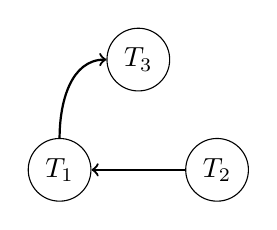
\begin{tikzpicture}
        [
            task/.style={circle, draw},
        ]
            \node[task] (T1) at (0.0, 0.0) {$T_1$};
            \node[task] (T2) at (2.0, 0.0) {$T_2$};
            \node[task] (T3) at (1.0, 1.4) {$T_3$};
            
            \draw[->, thick, draw] (T2.west) to [out=180,in=0] (T1.east);
            \draw[->, thick, draw] (T1.north) to [out=90,in=180] (T3.west);
        \end{tikzpicture}
        \caption{Precedence graph for schedule 1}
        \label{fig:trans-schedule-1}
    \end{figure}
    Since the graph is acyclic, schedule 1 is conflict serializable.

    \colbreak

    For schedule 2 we have that $T_3$ releases its locks before any other task
    wants to lock $Z$. Therefore, it is not dependent on any other task.
    Similarly, $T_1$ releases the lock on $Y$ before $T_2$ requests a lock on
    it. So they must also be independent. As there are no conflicts, the
    schedule is therefore inherently conflict serializable.
    \begin{figure}[H]
        \centering
        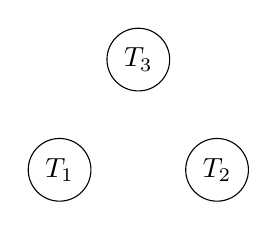
\begin{tikzpicture}
        [
            task/.style={circle, draw},
        ]
            \node[task] (T1) at (0.0, 0.0) {$T_1$};
            \node[task] (T2) at (2.0, 0.0) {$T_2$};
            \node[task] (T3) at (1.0, 1.4) {$T_3$};
        \end{tikzpicture}
        \caption{Precedence graph for schedule 2}
        \label{fig:trans-schedule-2}
    \end{figure}

\end{multicols}
